\chapter{Building Envelope Form Generation and Thermal Optimisation}

\section{Methodology of Thermal Optimisation and Form Generation}

The information presented so far requires at this point that a clear methodology, properly sequenced, and categorised, formulated out of the concepts and tools illustrated so far in the thesis.

To recapitulate the purpose of the thesis; the aim is to provide a practical method, sufficiently supported by previous experimentation, of designing a building envelope which meets the thermal performance criteria of the designer, through iterative environmental simulation and algorithmic optimisation, algorithmic form generation and regeneration.

The proposed procedure to guide such and endeavour, is based on the elements of the process described in the previous chapters, but differs in sequence to suite the natural order of the design process, and it is as follows:

\begin{enumerate}
	\item Analysis of envelope form
	\item Determination of thermal criteria
	\item Selection of suitable digital simulation and modelling environment
	\item Selection of suitable form generation and/or optimisation algorithms
\end{enumerate}

\paragraph{Introduction of Algorithmic Input to Design Process} \mbox{}

An important issue to be considered is the point at which algorithm is introduced to the design process. The introduction of algorithm (and simulation for that matter) at a very early stage as opposed to at a point when the schematic design has been almost finished would greatly influence the final product; as the former is considered pure form generation governed by optimisation algorithms, while the latter is considered optimisation of a geometry which has already been defined by the architect, and in turn defining the major optimisable variables.

Although the above would suggest that algorithmic form generation is best introduced at the earliest stage possible, this is not practical as it would mean that endless possibilities can be explored with no regard to user requirements. Therefore, for the sake of simplicity and practicality, it has been assumed that a conceptual form has been designed and used as a basis for further algorithmic optimisation. Form generation in this case is mostly \emph{regeneration} of the modelled geometry representing the building envelope.

\paragraph{Multi-criterion Optimisation} \mbox{}

Many of the cases presented in chapter 4 have showcased optimisation of envelopes with regard to only one variable; i.e. single-criterion optimisation (albeit with the exceptions of sections such as \ref{sec:KendallPavilion}), which was for the sake of making a clear and simple illustration of one concept or another. However, thermal optimisation in real world will almost always demand optimisation with more than one variable taken into consideration.

New problems will present themselves when shifting from single to multiple criterion optimisation, but by far the most important and influential is the problem of \emph{variable weighting system}, which is essentially the importance of each variable (external shading, fenestration\ldots etc.) in relation to the other variables. This should be studied and planned carefully by the architect, as conflicting variables will often demand very different solutions for each to be at optimum performance, and therefore the effect of each on the overall performance should be studied by the architect, possibly with the support of modelling and environmental simulation programs.

Another solution which in some cases might be practical, is to create reference points within the architectural space from which to measure the overall performance of the building envelope regardless of each variable and be used as the driving force behind the optimisation algorithm.

\subsection{Analysis and Categorisation of Envelope Form}

As described earlier (see page \pageref{BuildEnvDef}), any building envelope is composed of the architectural physical elements that separate the inside from the outside, creating an \emph{envelope} or \emph{enclosure} for the building.

Although this definition applies to almost all building envelopes, they would vary greatly from one building to another, making the task at hand; which is the utilisation of algorithmic design and thermal simulation to achieve thermally efficient buildings, inefficient or even practically meaningless, unless proper categorisation of building envelope design is made.

This is due to the fact that with differences between building enclosure designs, the variables that affect the thermal performance of the envelope will have varying degrees of impact, sometimes even reaching almost zero impact in some cases; having mentioned above the importance of weighting in multi-criterion optimisation, this would especially important to determine which variable should be given the priority over others.

\paragraph{\emph{Phylogenesis} and the Categorisation of Building Envelopes}\mbox{}

One interesting way of categorising building enclosures, is the endeavour undertaken by the \emph{Foreign Office Architects} to categorise their own work in a book named \emph{Phylogenesis: FOA's Ark} \cite{foa04}. The categorisation system resembles a biological evolutionary tree, that starts from one point and branches into different species through several evolutionary stages (figures \ref{fig:Phylogenesis} and \ref{fig:FOAEnvelopes}).

Regardless of the concept, the categorisation of building envelopes used by the Foreign Office Architects (FOA), makes an excellent working ground for analysis of different envelope forms, and defining the the thermal variables and their level of importance.

\begin{sidewaysfigure}[htbp]
	\centering
	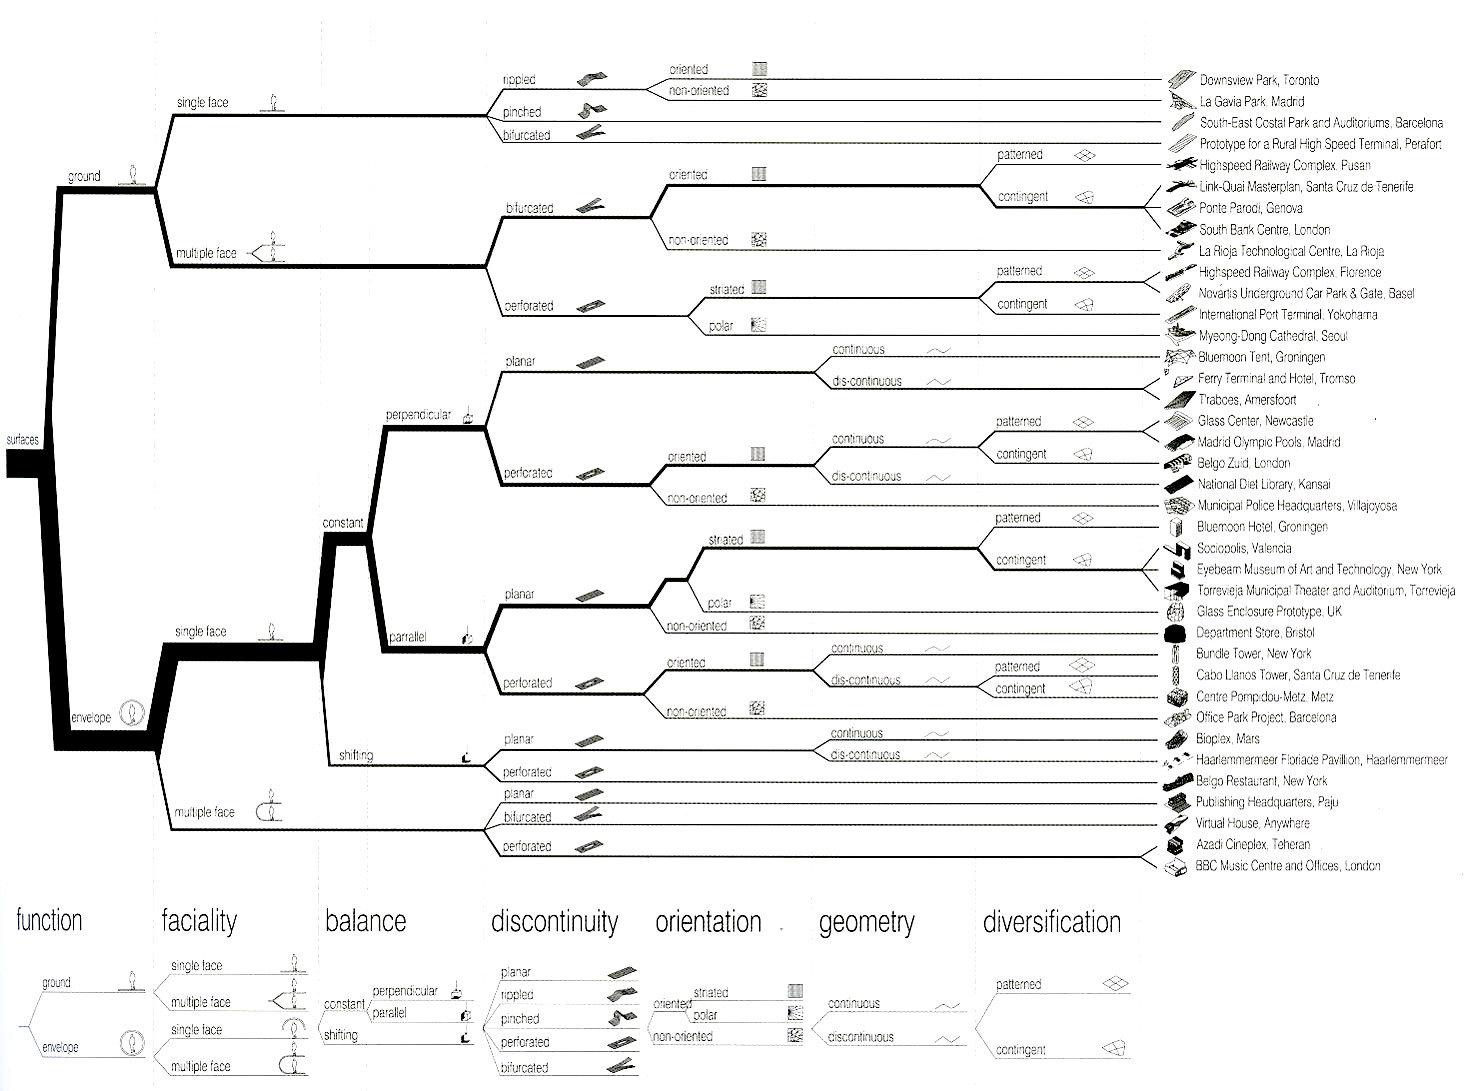
\includegraphics[width=20cm]{./Images/1-Phylogenesis}
	\caption[FOA Phylogenesis]{Structures Categorisation of FOA Work, Including Envelope Categorisation According to \emph{Phylogenesis} \cite{foa04}}
	\label{fig:Phylogenesis}
\end{sidewaysfigure}

\begin{figure}[H]
	\centering
	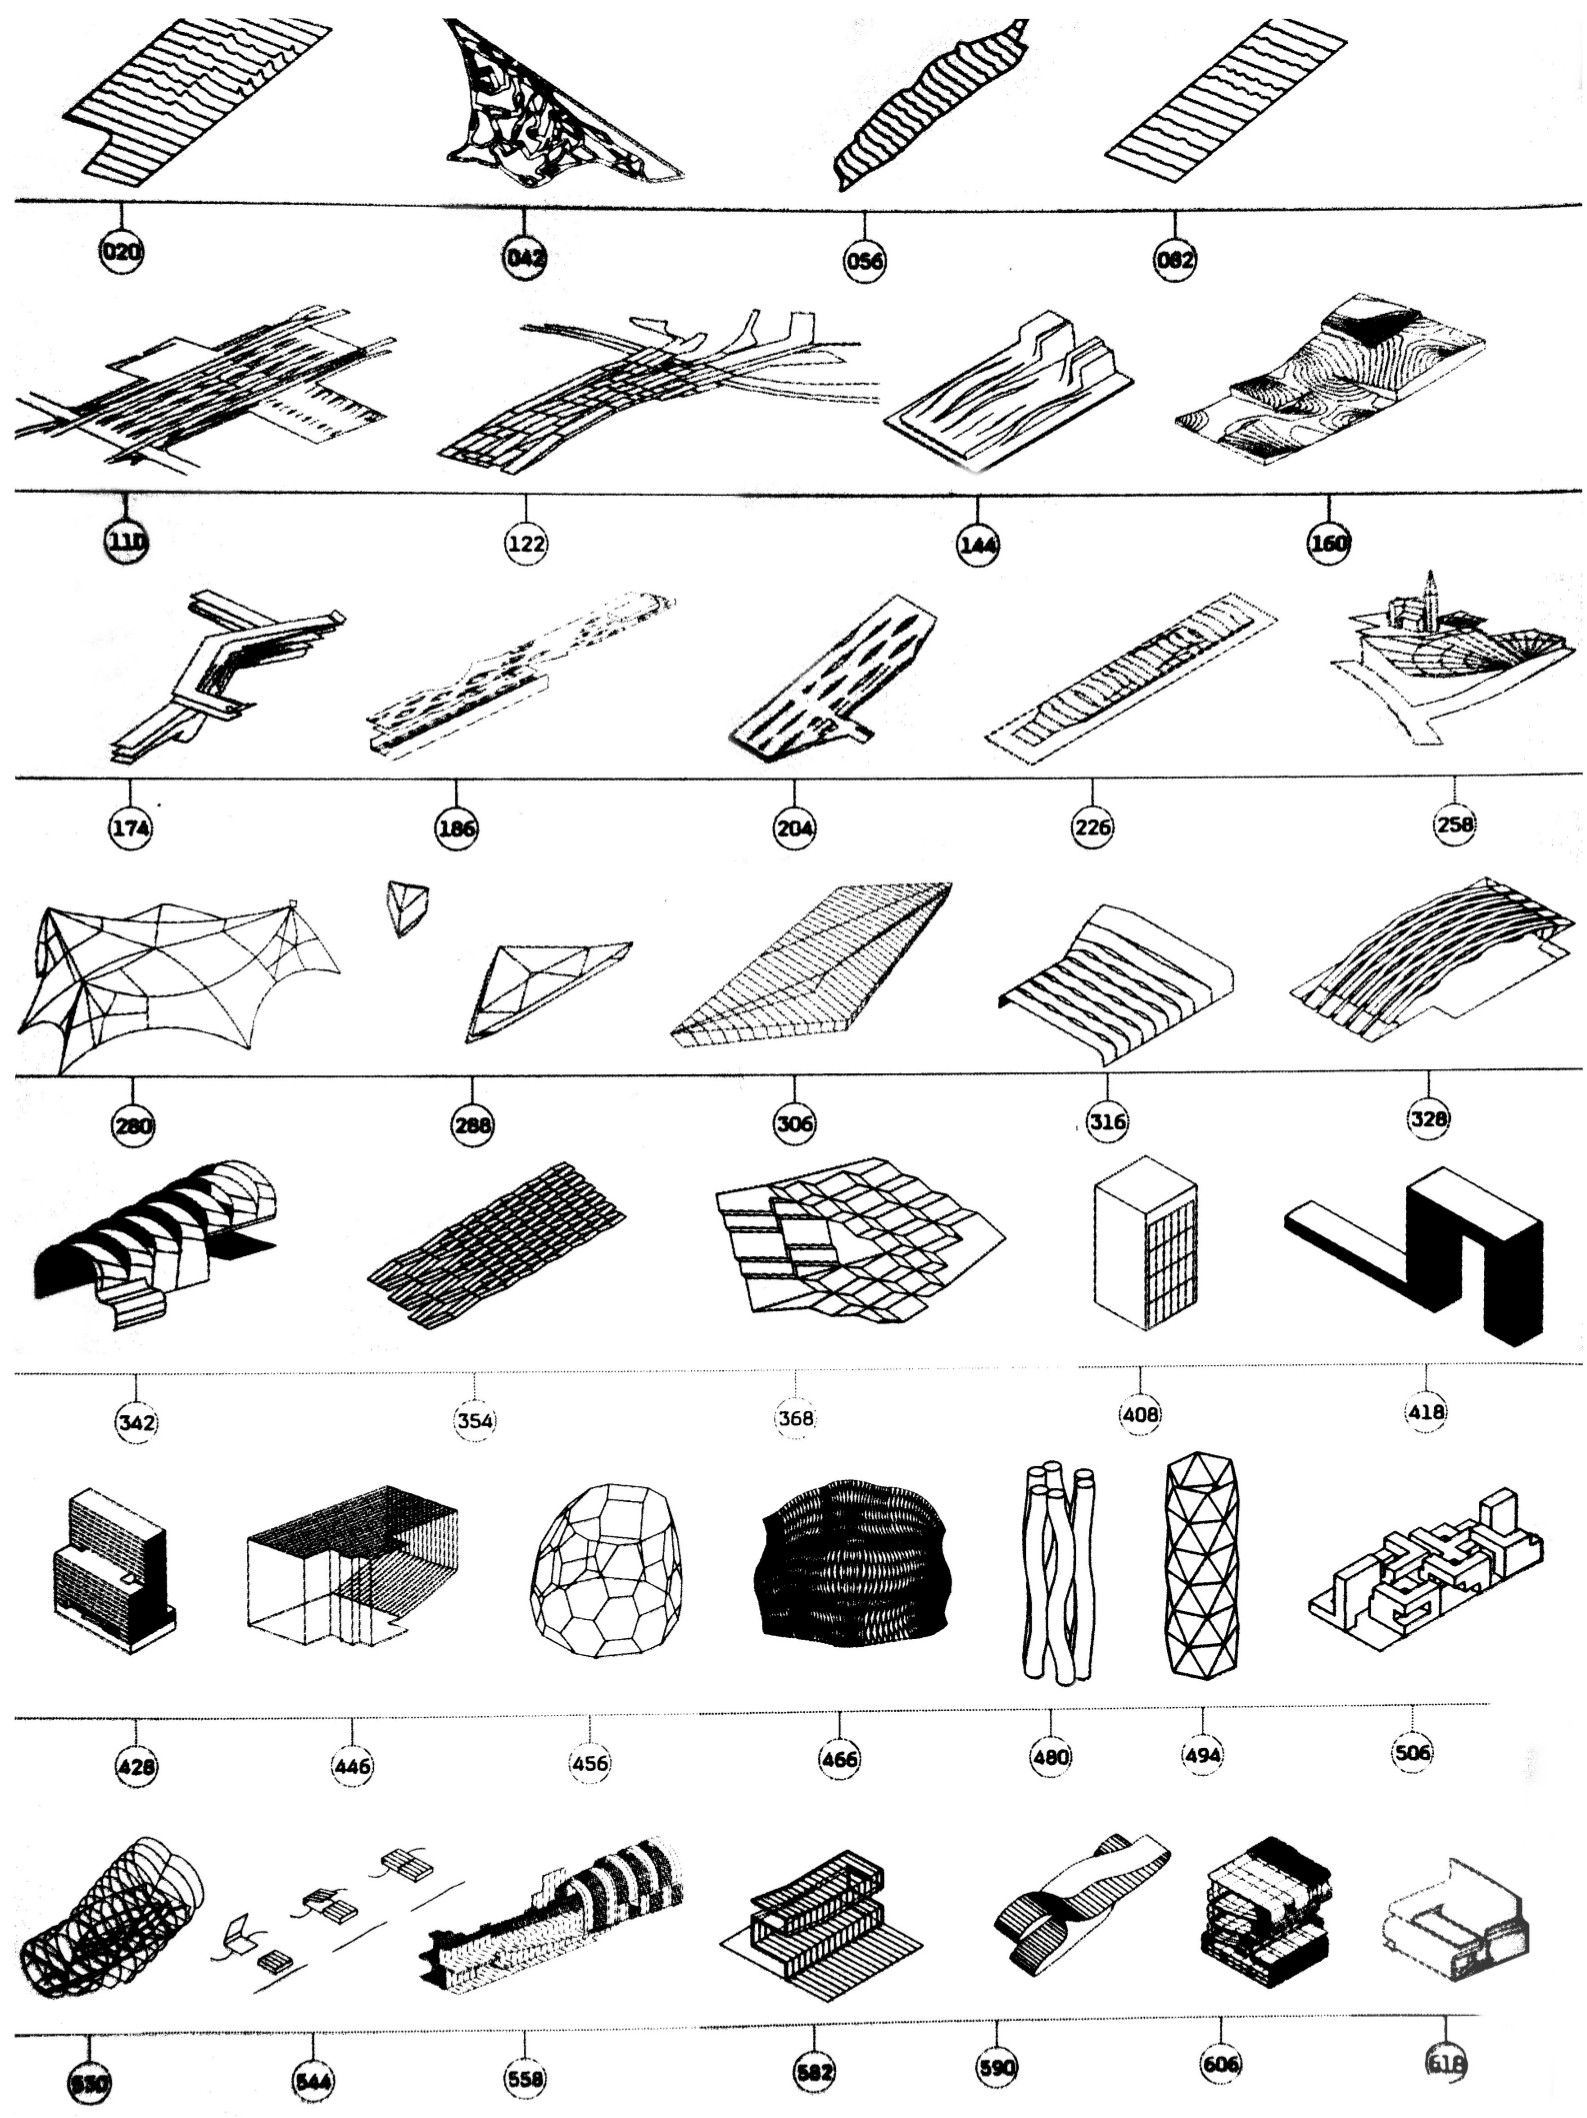
\includegraphics[width=\textwidth]{./Images/2-Envelopes}
	\caption[FOA Building Envelopes]{Examples of Structures and Building Envelopes by FOA \cite{foa04}}
	\label{fig:FOAEnvelopes}
\end{figure}


\subsection{Determination of Thermal Criteria}

Having created a system of categorisation in which any envelope form can mostly fit under a category; the thermal design through algorithm and simulation should be guided by the variables that affect the particular envelope form the most.

Here we refer to the design variables listed earlier in Chapter 3 (see page \pageref{sec:ThermalDesignVariables}), which are concerned with thermal design through passive solar control. This holds true in Chapter 4 as well, and has been done as such with the intention of simplifying the process and narrowing the scope for easier but effective illustration of the concepts throughout the thesis.

For the sake of convenience, the variables are re-listed here in table form.

\begin{table}[H]
	\centering
	\begin{tabular}{l|l}
		\textbf{Shape}		&Surface-to-Volume Ratio\\
					&Orientation\\
					&\\
		\textbf{Fabric} 	&Shading\\
					&Surface Material Properties\\
					&\\
		\textbf{Fenestration}	&Size, Position and Orientation\\
					&Glazing Material\\
					&Closing Mechanism\\
					&External Shading\\
	\end{tabular}
	\caption{Thermal Design Variables}
	\label{tab:ThermalDesignVariables}
\end{table}

\subsubsection{Building Envelope Form and Variables}

Before proceeding with assigning variables as driving parameters in the algorithmic design process, the above stated variables must be further explained with illustrative examples (it is advised to refer to the material presented in Chapter 3, as this section is concerned only with the practical aspect of analysing building envelopes in terms of thermal design variables).

\paragraph{Surface-to-Volume Ratio}\mbox{}

The surface-to-volume ratio of any building is mainly affected by three factors:

\begin{enumerate}
	\item Envelope Geometry; such as cubic, dome-shaped, spherical, pyramid-shaped\ldots{}etc (figure \ref{fig:SVR}).
		\begin{figure}[H]
			\centering
			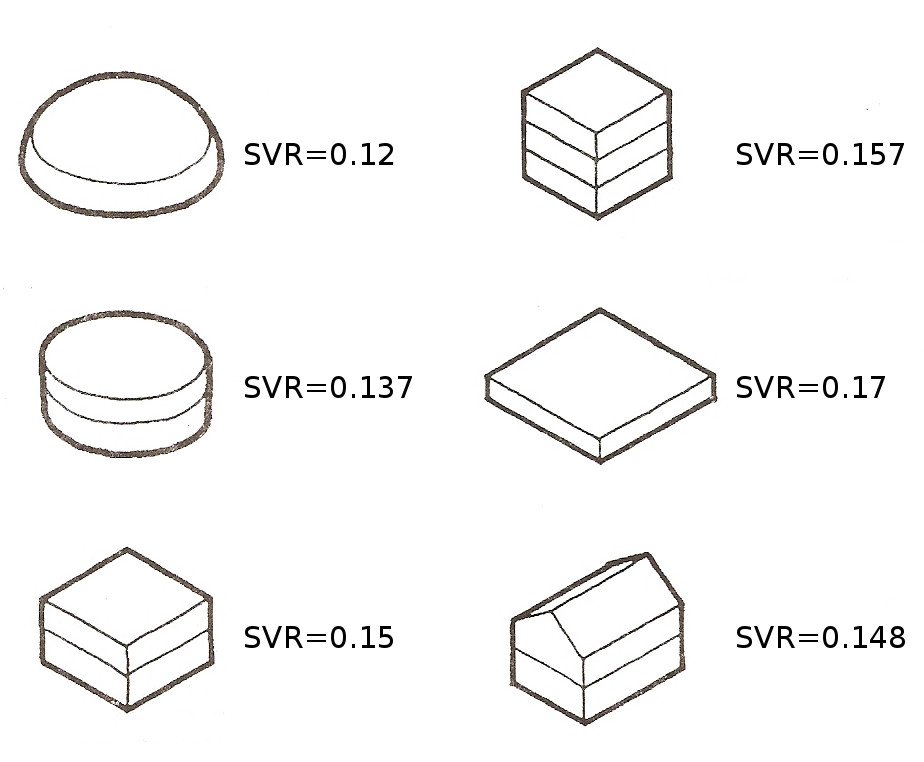
\includegraphics[width=\textwidth]{./Images/3-SVR}
			\caption{Surface-to-Volume Ratios}
			\label{fig:SVR}
		\end{figure}
	\item Compaction of Building Shape; with the same basic building shape, the SVR can be decreased using compaction, or greatly increased with		  lack of it (figure \ref{fig:Compaction}).
		\begin{figure}[H]
			\centering
			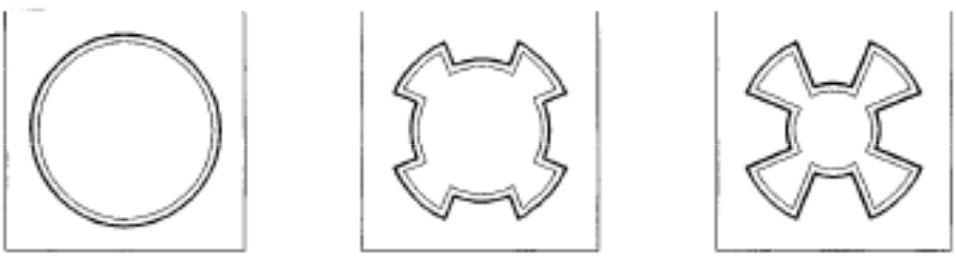
\includegraphics[width=\textwidth]{./Images/4-Compaction}
			\caption{Building Envelope Compaction}
			\label{fig:Compaction}
		\end{figure}
	\item Porosity; inner courts can create what may be called porosity of building envelope, which increases surface to volume ratio (figure 		\ref{fig:Porosity}).
		\begin{figure}[H]
			\centering
			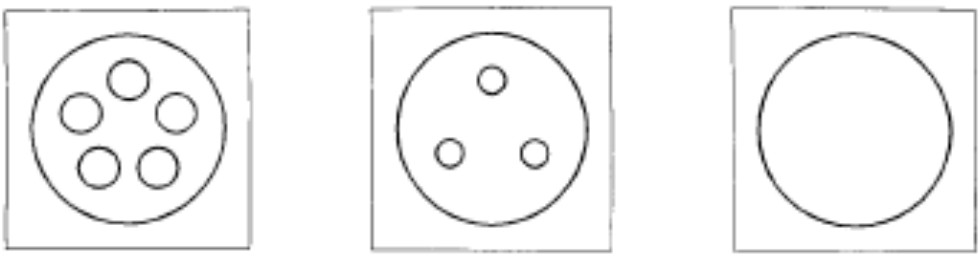
\includegraphics[width=\textwidth]{./Images/5-Porosity}
			\caption{Building Envelope Porosity}
			\label{fig:Porosity}
		\end{figure}
\end{enumerate}

\paragraph{Orientation}\mbox{}

Building orientation affects thermal performance mainly in two ways:
\begin{enumerate}
	\item The way the building perceives incident solar rays, which is dependant on the latitude of the location, and building envelope form. It should be noted that in some cases the effect of orientation is limited only to internal functions being performed in internal spaces facing a specific orientation. Buildings that are affected the most by their orientation are the ones that have big length to width ratio ---or elongated forms--- or highly non-uniform forms. (figure \ref{fig:orientation}).
		\begin{figure}[H]
			\centering
			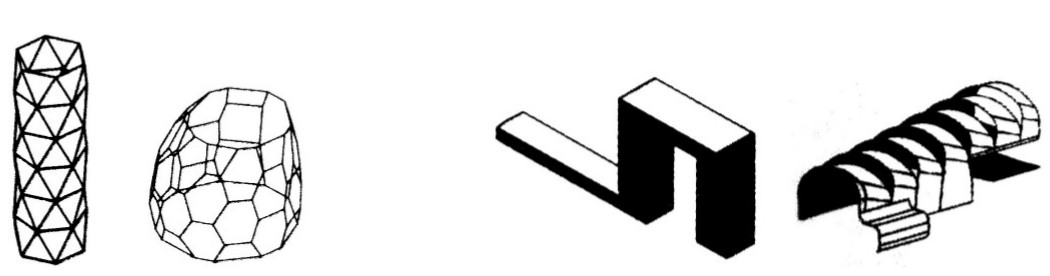
\includegraphics[width=13cm]{./Images/6-Orientation}
			\caption[Effect of Building Orientation]{In this example, the two buildings on the right would be greatly affected by their orientation in relation to the sun's position, while the two on the left are not affected except in terms of choosing internal space functions \cite{foa04}}
			\label{fig:orientation}
		\end{figure}
	\item Wind direction, which is not within the scope of this thesis.
\end{enumerate}

\paragraph{Shading}\mbox{}

What is referred to here as shading is the casting of shadow from the building onto itself; i.e. the obstruction of direct solar rays incidence on one part of the building using another.

Shading is closely related to orientation of the building, or even a direct result of it, however, it is not the only factor affecting it. The geometry of the building can greatly affect shading; an example would be part of the fa\c{c}ade which is a large cantilever hanging over lower floors (see the example in figure \ref{fig:ShadingCntlvr}).

\begin{figure}[H]
	\centering
	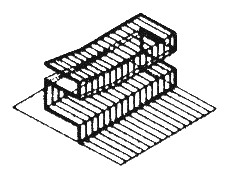
\includegraphics[width=7cm]{./Images/7-Cantilever}
	\caption[Envelope Shading]{A large part of the envelope can be facing the sun's direction but still be shaded under the cantilever parts of the building envelope \cite{foa04}}
	\label{fig:ShadingCntlvr}
\end{figure}

\paragraph{Surface Material Properties}\mbox{}

This is discussed at length in Chapter 3. Reference should be made to section \ref{sec:SolarHeatGain}, and the equation provided thereof as a basis for assigning parameters to materials such as reflectance, and to be iteratively modified through different generations of running the optimisation algorithm.

\paragraph{Fenestration Size, Shape and Position}\mbox{}

There have been several examples of the effect of opening size, shape and position on the thermal performance of a building envelope in the previous chapter, such as the Responsive Fa\c{c}ade Design System (see section \ref{sec:RFDS}) and the Generative System Method (see section \ref{sec:GSM}).

The size of fenestration is often constrained by the required amount of natural daylight for internal spaces, since both are inversely proportional. Position and shape are also important factors to be considered in the simulation.

Fenestration is almost always present in any building, however, with the exception of envelopes such as tent structures (figure \ref{fig:tent}). The absence of fenestration will render in most cases the following variables obsolete: \begin{inparaenum} \item Glazing Material, \item Closing Mechanism, and \item External Shading.\end{inparaenum}

\begin{figure}[H]
	\centering
	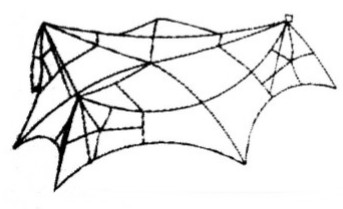
\includegraphics[width=8cm]{./Images/8-Tent}
	\caption[Tent Structure]{A tent structure as an example would not be affected by fenestration variables}
	\label{fig:tent}
\end{figure}
\paragraph{Glazing Material}\mbox{}

The same concept of surface material properties applies to glazing material; the necessity of inputting glazing material properties is that it greatly affects algorithms that specifically target openings for optimisation; in other words, if the openings are double or triple glazed, the opening size can be much larger with the same performance of a smaller opening with single clear glazing.

\paragraph{Closing Mechanisms}\mbox{}

This allows for options such as louvers to be introduced into the design to increase the thermal performance of the envelope while considerably widening the range of opening sizes above the target performance.

\paragraph{External Shading}\mbox{}

This form of shading is designed to protect internal spaces from unwanted solar rays entering through openings (i.e. fenestration). The different forms of external shading have been explained in Chapter 3 (refer to page \pageref{Shading}).

\subsection{Selection of Simulation and Modelling Environment}

Different simulation programs have been discussed relatively at length in Chapter 3 (section \ref{sec:SimulationPrograms}). The points to be considered when choosing a simulation program are as follows:

\begin{enumerate}
	\item The features and capabilities of each simulation program; the suitability of the provided list of features will depend on the kind of work being done. In case of an experiment with narrow scope and an interest in producing many results as a basis for statistical analysis (a good example being this thesis, which focuses on thermal performance of building envelopes through passive solar design), a program which is highly efficient in this particular task is preferable. This where comparative analysis studies such as the one shown earlier (see figure \ref{fig:SimProg1}, Table 2: \emph{Building Envelope, Daylight and Solar}) are very beneficial in determining which simulation programs have specific features to suite the work.

		Where the work being carried out is related to real-life projects, with interest in all aspects affecting the environmental performance of the building, it is usually the simulation program which covers most of the features shown in figures \ref{fig:SimProg1} and \ref{fig:SimProg2} is chosen.
	
	\item The ability to directly input programming code or script into the simulation programme. This was evident in Chapter 4, where the ability to use scripts and programming languages such as Lua or to input optimisation algorithms into the simulation programme is essential.
\end{enumerate}

\subsection{Selection of Form Generation and Optimisation Algorithms}

The main focus of this thesis is the utilisation of algorithm in architectural design, particularly in thermal design of building envelopes; and the subject has been discussed in several parts of the thesis from different points of view.

Another aspect of most importance at this point is knowing which algorithms are most suited to the needs of the architect. As seen in the previous chapters, algorithms have different concepts; many are derived from or simulate natural evolution and growth in one way or another, others are very visual in that they detect specific shapes and transform them according to some given rule, and so on. The algorithms shown in this thesis have all been proved useful in architectural design, and specifically in thermal design.

However, having reached this point, where different building envelopes have different priorities in terms of thermal design criteria, and preferences with regards to simulation and environmental modelling programmes, it is necessary to choose the most efficient algorithm for the job. Below are some of the main points to be considered.

\subsubsection{Generative or Performative Algorithms}

Although as mentioned earlier in this chapter, that starting a model from scratch would be troublesome and inefficient; it is also possible to define some basic parameters as a start, which would guide the form generating algorithm. One example would be Cellular Automata, which can create a building from scratch and therefore a building envelope form with the simple cell adjacency rules of Cellular Automata. In this case most generative algorithms would be useful.

Another case would be that a simple form exists, as designed by the architect, and requires optimisation and therefore requires adjustments to the existing envelope. This puts more control in the hand of the architect of the building envelope shape, but at the cost of less effectiveness of the optimisation algorithms, unless the algorithm has no or very few constraints which would allow it to perform extreme adjustments to the envelope form, to achieve the target performance. In this case optimisation or performative algorithms are useful.

\paragraph{Generative Algorithms}\mbox{}

\subparagraph{Control Constraints}

Each envelope form --- which is presumed to be at least conceptually defined to the point where it can be categorised under one of FOA envelope categories --- can be generated with different control techniques of the form evolution; this control comes in the form of constraints which are predefined by the algorithm use.

An example would be Shape Grammars; its constraints are colours, labaels and axis; while the constraints of Cellular Automata are state, neighbour and location\ldots and so on. So in order to control the evolution of the generated form, one must choose the most fitting method of control over the generating of envelope form.

The different constraints of each algorithm can be seen in table \ref{tab:GenerativeRecap}.

\subparagraph{Building Blocks and Unit Types}

The building blocks of different algorithms are the smallest units used by the algorithm; which is important since some algorithms might not be compatible with the desired forms. For example, Cellular Automata's building blocks are cells, while Shape Grammar's are basic shapes such as triangles\ldots{}etc.

It should be noted, that combinations of generative algorithms are possible, an example is shown as in figure \ref{3dCAArch}, where an algorithm similar to shape grammars is responsible for modifying the final result of cellular automata generations.

\paragraph{Performative Algorithms}\mbox{}

Many optimisation algorithms exist other than those discussed so far, but the heuristic optimisation algorithms are usually the fastest and are fairly efficient, at least as far architectural design is concerned, and in most cases of thermal design these are the primary concerns.

Upon studying the comparative analysis of performative algorithms (refer to table \ref{tab:OptCmp}), the main elements affecting the choice of algorithm would be as follows.

\subparagraph{Speed}

As mentioned earlier in the thesis, search methods such as \emph{Brute Force} would theoratically have a 100\% chance of locating the global optimum; however, this comes at the price of speed. Complex problems could take days or weeks to find the global optimum since it would need to try out all possible solutions within a solution space, which could be millions or virtually infinite.

Therefore, an algorithm that can find highly elite solutions within the solution space within a short time are always preferred. Generally speaking, of the three algorithms, \emph{Simulated Annaeling} is the fastest, followed by \emph{Genetic Algorithm} and then \emph{Tabu Search}.

\subparagraph{Architectural Alternatives}

When a purely engineering problem is being solved using a search method, the global optimum is usually the only concern. However, when the aesthetic aspect of the solution is of concern, such as in architectural solutions, the possibility of providing alternatives in the form of elite solutions is of very high importance.

Of the three algorithms, \emph{Genetic Algorithms} is the one that satisfies this need to the greatest extent.

\subparagraph{Search Efficiency}

Finding the optimum solutions is a prime concern, and therefore, the ability to locate as many of them and as close to the global optimum as possible is a major element to be considered in the choice of algorithm.

While \emph{Tabu Search} could be considered more efficient at locating optimum solutions, \emph{Genetic Algorithm} is almost equally as capable.


\clearpage
\section{Examples by Envelope Type}

At this point, the information provided so far in this chapter should be sufficient as a guide on how to design a thermally efficient building envelope using algorithm. The procedure has also been summarised for convinience in the following flowchart (figure \ref{fig:Ch5Flowchart}).

\begin{sidewaysfigure}[h]
	\centering
	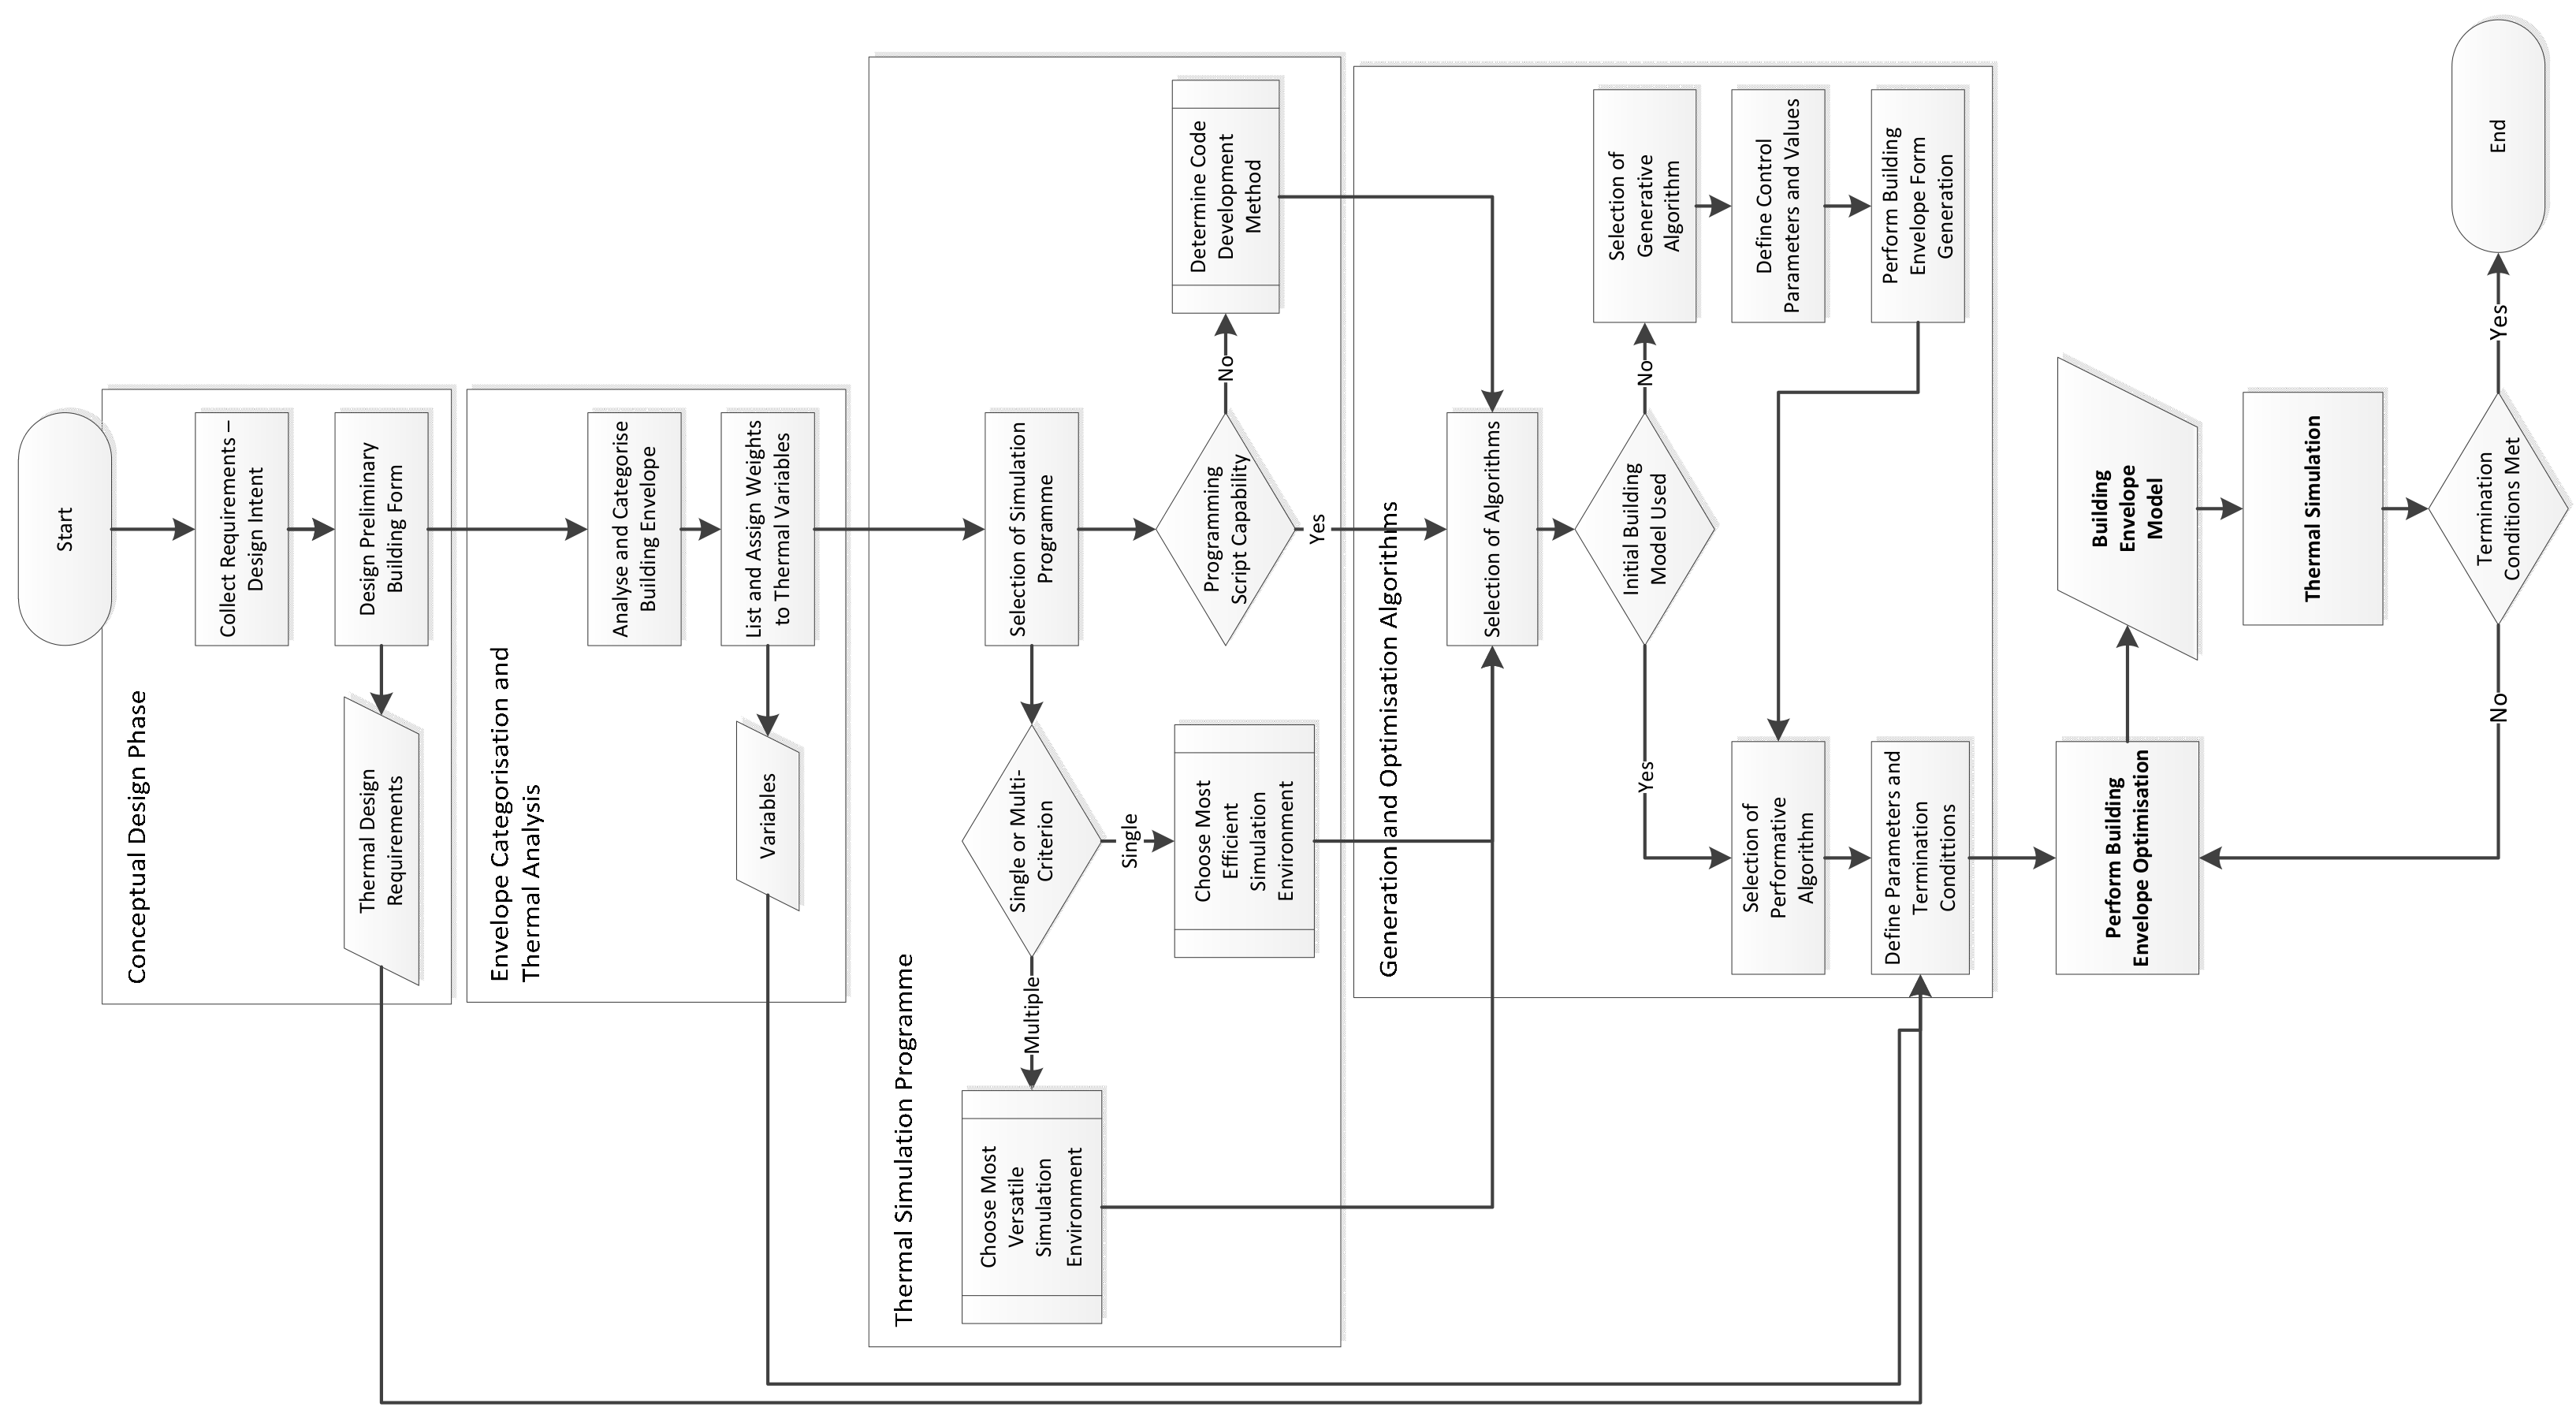
\includegraphics[width=21cm]{./Images/9-Flowchart}
	\caption[Thermal Algorithmic Design Flowchart]{Flowchart of procedure for thermal design using simulation programs and algorithms}
	\label{fig:Ch5Flowchart}
\end{sidewaysfigure}

Using the flowchart, a number of examples will be presented to show the different outcomes depending on the different envelope forms.

For each buidling envelope form ---which should be developed at the conceptual design phase of the chart--- the following have been listed:

\begin{enumerate}
	\item The most dominant thermal variables over building thermal performance for this particular envelope form
	\item The most suitable simulation programme based on the criteria given earlier in this chapter
	\item The most suitable generative algorithm capable of generating the form, if applicable or needed
	\item The most efficient or effective performative (optimisation) algorithm for the envelope form
	\item The buidling envelope species as categorised by FOA \cite{foa04}.
\end{enumerate}

\paragraph{Important Notes}\mbox{}

\begin{enumerate}
	\item In some cases where the selection of generative algorithm is stated as ``\emph{Not Applicable}'', this does not necessarily mean that no generative algorithm is capable of generating the particular envelope, only that the algorithms discussed are probably not suitable.
	\item The examples presented and the selected variables, programmes and algorithms are not undisputable. Experimentation is necessary for the succes of unique case of building envelope.
\end{enumerate}

\clearpage

\begin{sidewaystable}[h]
	\begin{tabular}{ | m{6cm} | m{14cm} |}
	\toprule
	\multicolumn{2}{c}{Envelope \#{}1} \\[1cm] \hline
	\multirow{7}{*}{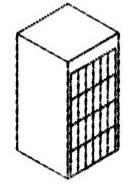
\includegraphics[width=5cm]{./Images/10-Envelope1}} & \textbf{Thermal Variables} \\[1cm]
	& Surface Material Properties | Fenestration SPO\footnote{Size, Position and Orientation} | Glazing Material | Closing Mechanism\vspace{0.5cm}\\ \cline{2-2}
		 & \textbf{Simulation Programme} \\[1cm]
		 & \emph{Solar Gain:} EnergyPlus | \emph{Economic Evaluation}: DOE-2.1E | \emph{Zone Loads:} ECOTECT | \emph{HVAC:} TRANSYS \vspace{0.5cm}\\ \cline{2-2}
		 & \textbf{Generative Algorithm} \\[1cm]
		 & \emph{Not Applicable}\vspace{0.5cm}\\ \cline{2-2}
		 & \textbf{Performative Algorithm} \\[1cm]
		 \emph{Ensifacopa Planorstripat} &  Tabu Search | Simulated Annaeling\vspace{0.5cm}\\
	\bottomrule
	\end{tabular}
\end{sidewaystable}

\clearpage

\begin{sidewaystable}[h]
	\begin{tabular}{ | m{6cm} | m{14cm} |}
	\toprule
	\multicolumn{2}{c}{Envelope \#{}2} \\[1cm] \hline
	\multirow{7}{*}{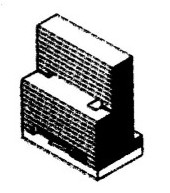
\includegraphics[width=5.5cm]{./Images/11-Envelope2}} & \textbf{Thermal Variables} \\[1cm]
	& Orientation | Shading | Glazing Material | Closing Mechanism\vspace{0.5cm}\\ \cline{2-2}
		 & \textbf{Simulation Programme} \\[1cm]
		 & \emph{Solar Gain:} EnergyPlus | \emph{Economic Evaluation}: DOE-2.1E | \emph{Zone Loads:} ECOTECT | \emph{HVAC:} TRANSYS \vspace{0.5cm}\\ \cline{2-2}
		 & \textbf{Generative Algorithm} \\[1cm]
		 & \emph{Not Applicable}\vspace{0.5cm}\\ \cline{2-2}
		 & \textbf{Performative Algorithm} \\[1cm]
		 \emph{Ensifacopa Planorstricon Oculus} &  Tabu Search\vspace{0.5cm}\\
	\bottomrule
	\end{tabular}
\end{sidewaystable}

\begin{sidewaystable}[h]
	\begin{tabular}{ | m{6cm} | m{14cm} |}
	\toprule
	\multicolumn{2}{c}{Envelope \#{}3} \\[1cm] \hline
	\multirow{7}{*}{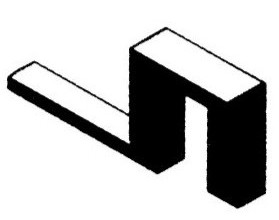
\includegraphics[width=5.5cm]{./Images/12-Envelope3}} & \textbf{Thermal Variables} \\[1cm]
		& Surface-to-Volume Ratio | Orientation | Shading\vspace{0.5cm}\\ \cline{2-2}
	 	& \textbf{Simulation Programme} \\[1cm]
	 	& \emph{solar gain:} energyplus | \emph{economic evaluation}: doe-2.1e | \emph{zone loads:} ecotect | \emph{hvac:} transys \vspace{0.5cm}\\ \cline{2-2}
	 	& \textbf{Generative Algorithm} \\[1cm]
	 	& L-System\vspace{0.5cm}\\ \cline{2-2}
	 	& \textbf{Performative Algorithm} \\[1cm]
	 	\emph{Ensifacopa Planorstricon Socio} &  Genetic Algorithm\vspace{0.5cm}\\
\bottomrule
\end{tabular}
\end{sidewaystable}

\clearpage

\begin{sidewaystable}[h]
	\begin{tabular}{ | m{6cm} | m{14cm} |}
	\toprule
	\multicolumn{2}{c}{Envelope \#{}4} \\[1cm] \hline
	\multirow{7}{*}{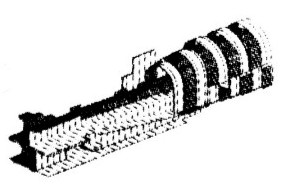
\includegraphics[width=5.5cm]{./Images/13-Envelope4}} & \textbf{Thermal Variables} \\[1cm]
	& Orientation | Surface Material Properties | External Shading\vspace{0.5cm}\\ \cline{2-2}
		 & \textbf{Simulation Programme} \\[1cm]
		 & \emph{Solar Gain:} Energyplus | \emph{Economic Evaluation}: DOE-2.1E | \emph{Zone Loads:} ECOTECT | \emph{HVAC:} TRANSYS \vspace{0.5cm}\\ \cline{2-2}
		 & \textbf{Generative Algorithm} \\[1cm]
		 & \emph{Not Applicable}\vspace{0.5cm}\\ \cline{2-2}
		 & \textbf{Performative Algorithm} \\[1cm]
		 \emph{Ensifashi Perfo} &  Genetic Algorithm\vspace{0.5cm}\\
	\bottomrule
	\end{tabular}
\end{sidewaystable}

\clearpage

\begin{sidewaystable}[h]
	\begin{tabular}{ | m{6cm} | m{14cm} |}
	\toprule
	\multicolumn{2}{c}{Envelope \#{}5} \\[1cm] \hline
	\multirow{7}{*}{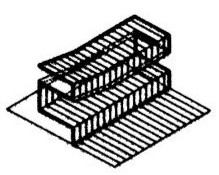
\includegraphics[width=5.4cm]{./Images/14-Envelope5}} & \textbf{Thermal Variables} \\[1cm]
	& Shading | Surface Material Properties | Glazing Material\vspace{0.5cm}\\ \cline{2-2}
		 & \textbf{Simulation Programme} \\[1cm]
		 & \emph{Solar Gain:} EnergyPlus | \emph{Economic Evaluation}: DOE-2.1E | \emph{Zone Loads:} ECOTECT | \emph{HVAC:} TRANSYS \vspace{0.5cm}\\ \cline{2-2}
		 & \textbf{Generative Algorithm} \\[1cm]
		 & L-System | Shape Grammars\vspace{0.5cm}\\ \cline{2-2}
		 & \textbf{Performative Algorithm} \\[1cm]
		 \emph{Enmulfa Plana} &  Genetic Algorithm\vspace{0.5cm}\\
	\bottomrule
	\end{tabular}
\end{sidewaystable}

\clearpage

\begin{sidewaystable}[h]
	\begin{tabular}{ | m{6cm} | m{14cm} |}
	\toprule
	\multicolumn{2}{c}{Envelope \#{}6} \\[1cm] \hline
	\multirow{7}{*}{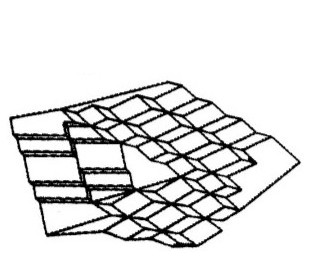
\includegraphics[width=5.5cm]{./Images/15-Envelope6}} & \textbf{Thermal Variables} \\[1cm]
	& Surface-to-Volume Ratio | Surface Material Properties \vspace{0.5cm}\\ \cline{2-2}
		 & \textbf{Simulation Programme} \\[1cm]
		 & \emph{Solar Gain:} EnergyPlus | \emph{Economic Evaluation}: DOE-2.1E | \emph{Zone Loads:} ECOTECT | \emph{HVAC:} TRANSYS \vspace{0.5cm}\\ \cline{2-2}
		 & \textbf{Generative Algorithm} \\[1cm]
		 & Fractals | Shape Grammars\vspace{0.5cm}\\ \cline{2-2}
		 & \textbf{Performative Algorithm} \\[1cm]
		 \emph{Ensifacoper Pernonor} &  Simulated Annaeling\vspace{0.5cm}\\
	\bottomrule
	\end{tabular}
\end{sidewaystable}

\clearpage

\begin{sidewaystable}[h]
	\begin{tabular}{ | m{6cm} | m{14cm} |}
	\toprule
	\multicolumn{2}{c}{Envelope \#{}7} \\[1cm] \hline
	\multirow{7}{*}{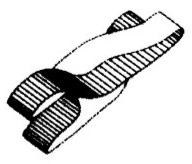
\includegraphics[width=5.3cm]{./Images/16-Envelope7}} & \textbf{Thermal Variables} \\[1cm]
	& Orientation | Shading | Surface Material Properties\vspace{0.5cm}\\ \cline{2-2}
		 & \textbf{Simulation Programme} \\[1cm]
		 & \emph{Solar Gain:} EnergyPlus | \emph{Economic Evaluation}: DOE-2.1E | \emph{Zone Loads:} ECOTECT | \emph{HVAC:} TRANSYS \vspace{0.5cm}\\ \cline{2-2}
		 & \textbf{Generative Algorithm} \\[1cm]
		 & \emph{Not Applicable}\vspace{0.5cm}\\ \cline{2-2}
		 & \textbf{Performative Algorithm} \\[1cm]
		 \emph{Enmulfa Bifur} &  Genetic Algorithm\vspace{0.5cm}\\
	\bottomrule
	\end{tabular}
\end{sidewaystable}

\clearpage

\begin{sidewaystable}[h]
	\begin{tabular}{ | m{6cm} | m{14cm} |}
	\toprule
	\multicolumn{2}{c}{Envelope \#{}8} \\[1cm] \hline
	\multirow{7}{*}{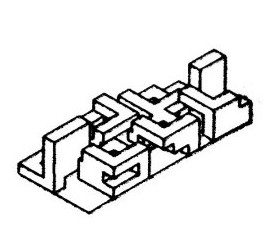
\includegraphics[width=5.2cm]{./Images/17-Envelope8}} & \textbf{Thermal Variables} \\[1cm]
	& Surface-to-Volume Ratio | Orientation | Shading\vspace{0.5cm}\\ \cline{2-2}
		 & \textbf{Simulation Programme} \\[1cm]
		 & \emph{Solar Gain:} EnergyPlus | \emph{Economic Evaluation}: DOE-2.1E | \emph{Zone Loads:} ECOTECT | \emph{HVAC:} TRANSYS \vspace{0.5cm}\\ \cline{2-2}
		 & \textbf{Generative Algorithm} \\[1cm]
		 & Cellular Automata\vspace{0.5cm}\\ \cline{2-2}
		 & \textbf{Performative Algorithm} \\[1cm]
		 \emph{Ensifacopa Pernonor Zonafranca} & Genetic Algorithm | Tabu Search \vspace{0.5cm}\\
	\bottomrule
	\end{tabular}
\end{sidewaystable}

\clearpage

\begin{sidewaystable}[h]
	\begin{tabular}{ | m{6cm} | m{14cm} |}
	\toprule
	\multicolumn{2}{c}{Envelope \#{}9} \\[1cm] \hline
	\multirow{7}{*}{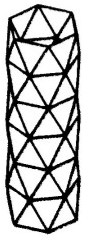
\includegraphics[height=5.5cm]{./Images/18-Envelope9}} & \textbf{Thermal Variables} \\[1cm]
	& Surface Material Properties | Glazing Material \vspace{0.5cm}\\ \cline{2-2}
		 & \textbf{Simulation Programme} \\[1cm]
		 & \emph{Solar Gain:} EnergyPlus | \emph{Economic Evaluation}: DOE-2.1E | \emph{Zone Loads:} ECOTECT | \emph{HVAC:} TRANSYS \vspace{0.5cm}\\ \cline{2-2}
		 & \textbf{Generative Algorithm} \\[1cm]
		 & Veronoi Diagram\vspace{0.5cm}\\ \cline{2-2}
		 & \textbf{Performative Algorithm} \\[1cm]
		 \emph{Ensifacopa Perordis} &  Tabu Search\vspace{0.5cm}\\
	\bottomrule
	\end{tabular}
\end{sidewaystable}

\clearpage

\begin{sidewaystable}[h]
	\begin{tabular}{ | m{6cm} | m{14cm} |}
	\toprule
	\multicolumn{2}{c}{Envelope \#{}10} \\[1cm] \hline
	\multirow{7}{*}{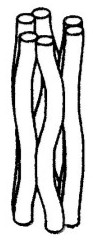
\includegraphics[height=5.5cm]{./Images/19-Envelope10}} & \textbf{Thermal Variables} \\[1cm]
	& Surface Material Properties | Shading | Glazing Material\vspace{0.5cm}\\ \cline{2-2}
		 & \textbf{Simulation Programme} \\[1cm]
		 & \emph{Solar Gain:} EnergyPlus | \emph{Economic Evaluation}: DOE-2.1E | \emph{Zone Loads:} ECOTECT | \emph{HVAC:} TRANSYS \vspace{0.5cm}\\ \cline{2-2}
		 & \textbf{Generative Algorithm} \\[1cm]
		 & L-System\vspace{0.5cm}\\ \cline{2-2}
		 & \textbf{Performative Algorithm} \\[1cm]
		 \emph{Ensifacopa Peroricon} &  Genetic Algorithm\vspace{0.5cm}\\
	\bottomrule
	\end{tabular}
\end{sidewaystable}

\clearpage

\begin{sidewaystable}[h]
	\begin{tabular}{ | m{6cm} | m{14cm} |}
	\toprule
	\multicolumn{2}{c}{Envelope \#{}11} \\[1cm] \hline
	\multirow{7}{*}{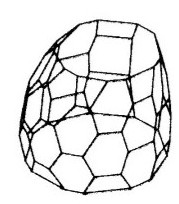
\includegraphics[width=5cm]{./Images/20-Envelope11}} & \textbf{Thermal Variables} \\[1cm]
	& Surface-to-Volume Ratio | Surface Material Properties | Glazing Material\vspace{0.5cm}\\ \cline{2-2}
		 & \textbf{Simulation Programme} \\[1cm]
		 & \emph{Solar Gain:} EnergyPlus | \emph{Economic Evaluation}: DOE-2.1E | \emph{Zone Loads:} ECOTECT | \emph{HVAC:} TRANSYS \vspace{0.5cm}\\ \cline{2-2}
		 & \textbf{Generative Algorithm} \\[1cm]
		 & Veronoi Diagram\vspace{0.5cm}\\ \cline{2-2}
		 & \textbf{Performative Algorithm} \\[1cm]
		 \emph{Ensifacopa Planorpol} &  Genetic Algorithm | Simulated Annaeling\vspace{0.5cm}\\
	\bottomrule
	\end{tabular}
\end{sidewaystable}

\clearpage

\begin{sidewaystable}[h]
	\begin{tabular}{ | m{6cm} | m{14cm} |}
	\toprule
	\multicolumn{2}{c}{Envelope \#{}12} \\[1cm] \hline
	\multirow{7}{*}{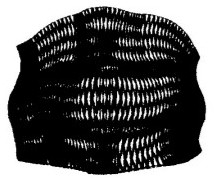
\includegraphics[width=5.5cm]{./Images/21-Envelope12}} & \textbf{Thermal Variables} \\[1cm]
	& Surface-to-Volume Ratio | Shading | Glazing Material | Closing Mechanism\vspace{0.5cm}\\ \cline{2-2}
		 & \textbf{Simulation Programme} \\[1cm]
		 & \emph{Solar Gain:} EnergyPlus | \emph{Economic Evaluation}: DOE-2.1E | \emph{Zone Loads:} ECOTECT | \emph{HVAC:} TRANSYS \vspace{0.5cm}\\ \cline{2-2}
		 & \textbf{Generative Algorithm} \\[1cm]
		 & Shape Grammars | Fractals\vspace{0.5cm}\\ \cline{2-2}
		 & \textbf{Performative Algorithm} \\[1cm]
		 \emph{Ensifacopa Planonor} &  Tabu Search\vspace{0.5cm}\\
	\bottomrule
	\end{tabular}
\end{sidewaystable}

\clearpage

\begin{sidewaystable}[h]
	\begin{tabular}{ | m{6cm} | m{14cm} |}
	\toprule
	\multicolumn{2}{c}{Envelope \#{}13} \\[1cm] \hline
	\multirow{7}{*}{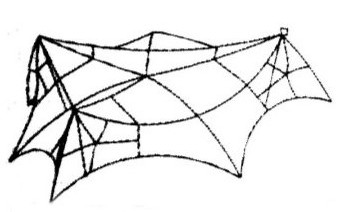
\includegraphics[width=5.5cm]{./Images/22-Envelope13}} & \textbf{Thermal Variables} \\[1cm]
	& Surface-to-Volume Ratio | Surface Material Properties | Shading\vspace{0.5cm}\\ \cline{2-2}
		 & \textbf{Simulation Programme} \\[1cm]
		 & \emph{Solar Gain:} EnergyPlus | \emph{Economic Evaluation}: DOE-2.1E | \emph{Zone Loads:} ECOTECT | \emph{HVAC:} TRANSYS \vspace{0.5cm}\\ \cline{2-2}
		 & \textbf{Generative Algorithm} \\[1cm]
		 & Shape Grammars\vspace{0.5cm}\\ \cline{2-2}
		 & \textbf{Performative Algorithm} \\[1cm]
		 \emph{Ensifacoper Placon} &  Simulated Annaeling | Genetic Algorithm\vspace{0.5cm}\\
	\bottomrule
	\end{tabular}
\end{sidewaystable}

\clearpage


